\begin{figure}[!htbp]
    \centering
    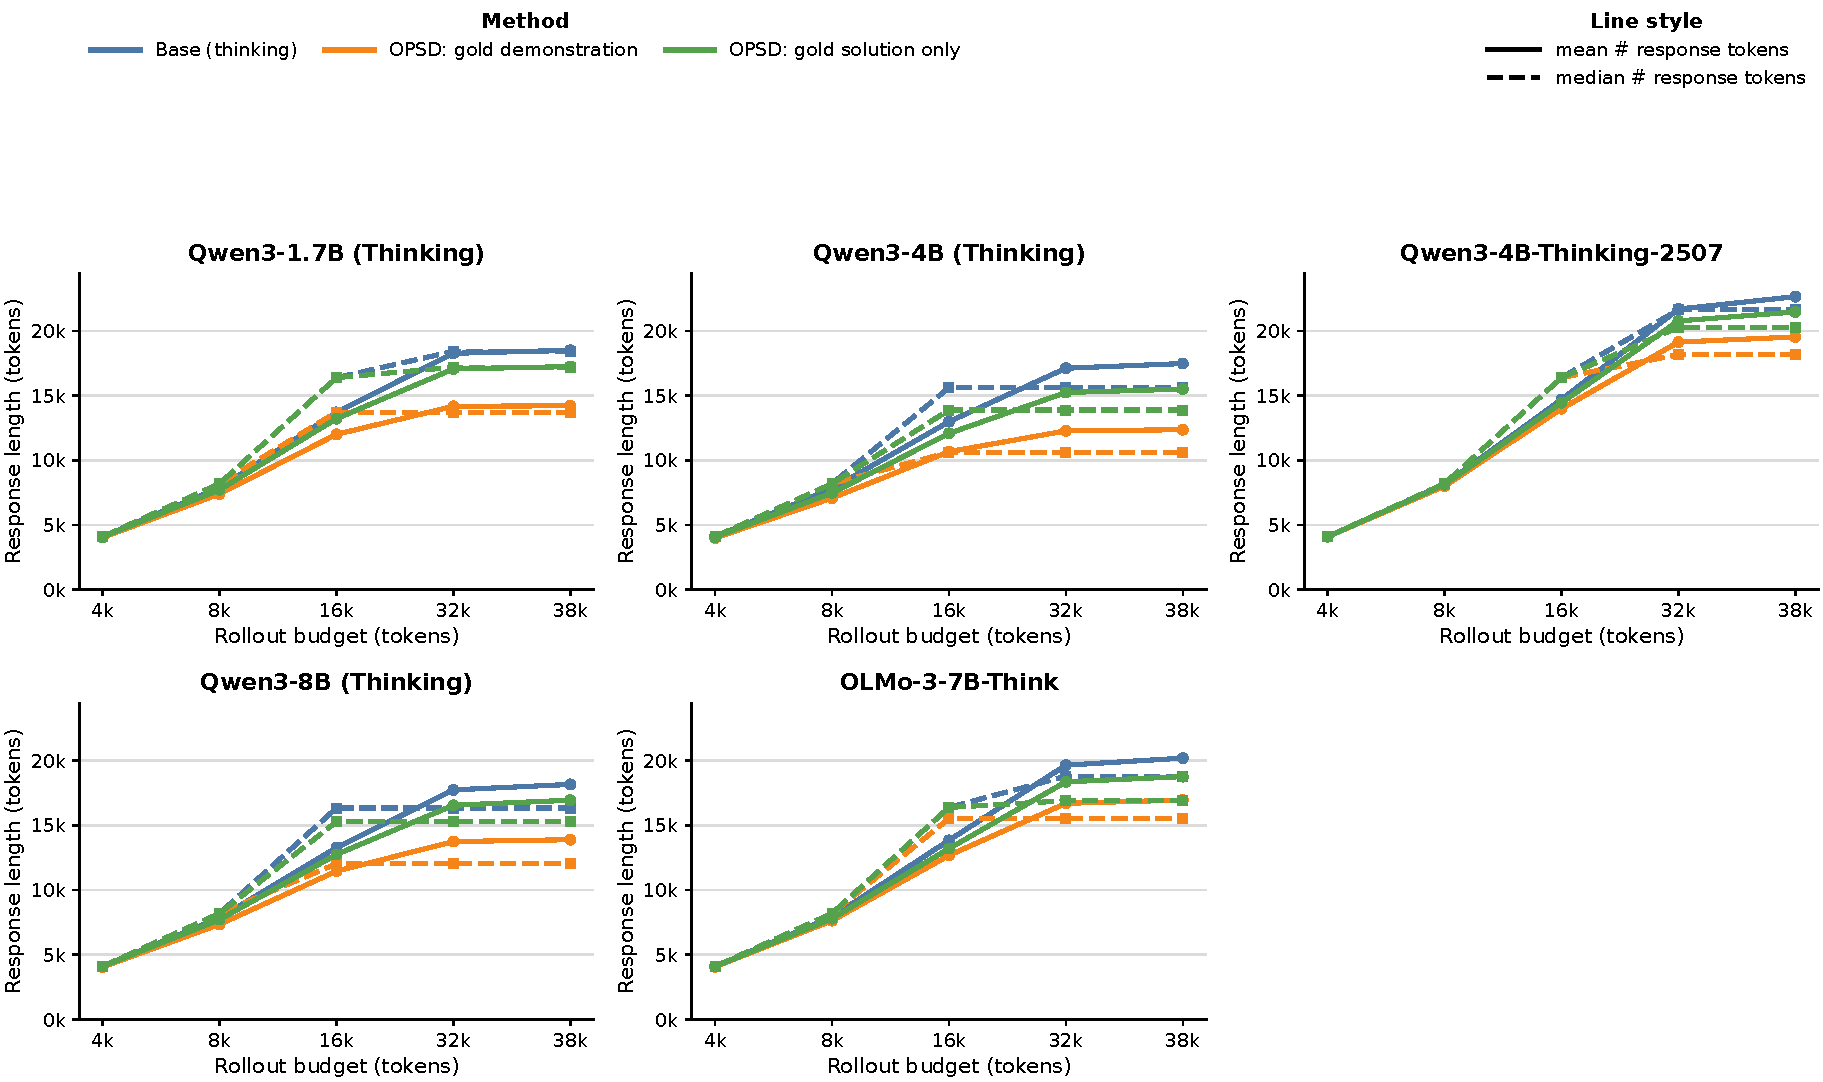
\includegraphics[width=\linewidth]{figures/avg_rollout_tokens_budget_curves_thinking5_fs_ao.pdf}
    \caption{
    \textbf{Per-model response-length budget curves show where \opsd{} compresses long thinking rollouts.}
    This companion to Figure~\ref{fig:openthoughts_accuracy_length_collapse} reports response-token counts for the same five OpenThoughts-trained thinking models, evaluation benchmarks, and rollout budgets as Figure~\ref{fig:openthoughts_budget_pass_rates_thinking5_fs_ao}.
    Solid lines show mean response length and dashed lines show median response length.
    Blue curves are base thinking models, orange curves are \opsd{} with full gold-demonstration context, and green curves are \opsd{} with final-answer-only privileged context.
    At 32k--38k token budgets, full-demonstration \opsd{} generally produces shorter responses than the corresponding base model.
    }
    \label{fig:openthoughts_budget_response_lengths_thinking5_fs_ao}
\end{figure}
